\documentclass[a4paper,10pt]{report}
\usepackage[utf8]{inputenc}
\usepackage{mathtools}

\begin{document}

\section*{Esboço}

Cada vértice tem:
\begin{itemize}
	\item $K_i$
	\item Histórico(id,$\sum_{tot}$) das suas comunidades
	\item Histórico das comunidades dos vizinhos
\end{itemize}
E para cada vizinho irá calcular o $K_{i,in}$ e o ganho em relação à comunidade do vizinho.


Então considerando o grafo na figura~\ref{fig:esb1}.

\begin{figure}
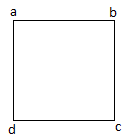
\includegraphics[width=20mm]{esboco1}
\caption{Primeiro grafo\label{fig:esb1}}
\end{figure}


\begin{table}[h]
	\centering
		\begin{tabular}{ l | l | l | l }
		\hline
			Vértice & Ki & Histórico Comunidades & Histórico Vizinhos \\ \hline
			a & 2 & (a,2) & - \\ \hline
			b & 2 & (b,2) & - \\ \hline
			c & 2 & (c,2) & - \\ \hline
			d & 2 & (d,2) & - \\ \hline
		\end{tabular}
\end{table}

Como o ganho (0.5) é igual para todos como regra de desempate os vértices escolhem a comunidade com o id menor, ficando cada vértice com os seguintes valores:

\begin{table}[h]
	\centering
		\begin{tabular}{ l | l | l | l }
		\hline
			Vértice & Ki & Histórico Comunidades & Histórico Vizinhos \\ \hline
			a & 2 & (a,2), (a,4) &  b: (b,2), d: (d,2)\\ \hline
			b & 2 & (b,2), (a,4) &  a: (a,2), c: (c,2)\\ \hline
			c & 2 & (c,2), (b,4) &  b: (b,2), d: (d,2)\\ \hline
			d & 2 & (d,2), (a,4) &  a: (a,2), c: (c,2)\\ \hline
		\end{tabular}
\end{table}

O que leva as três comunidades referidas na figura~\ref{fig:esb2}.

\begin{figure}
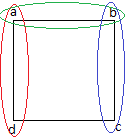
\includegraphics[width=20mm]{esboco2}
\caption{Primeiro grafo com as comunidades\label{fig:esb2}}
\end{figure}

Se no próximo passo cada vértice enviar para os seus vizinhos a sua comunidade atual e a comunidade dos seus outros vizinhos e ao receber esta informação decidir que, como o seu vizinho decidiu juntar-se a outra comunidade, irá também juntar-se a comunidade do vizinho atualizando o seu $\sum_{tot}$ de acordo. Faz isso para todos os vizinhos, ou seja, é feito uma união entre todas as comunidades.


No exemplo apresentado anteriormente basta enviar o histórico local dos vizinhos para garantir que o $\sum_{tot}$ da comunidade está atualizado em todos os vértices da comunidade. Podendo começar a enviar esta nova informação aos vizinhos não pertencentes à mesma comunidade e recomeçar.

\begin{figure}
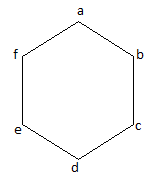
\includegraphics[width=20mm]{esboco3}
\caption{Segundo grafo\label{fig:esb3}}
\end{figure}

\newpage
 Mas referindo agora ao grafo na figura~\ref{fig:esb3}. Tal como no primeiro grafo o ganho (2/3) é igual para todos os vértices. E depois do primeiro cálculo cada vértice fica com os seguintes valores:

\begin{table}[h]
	\centering
		\begin{tabular}{ l | l | l | l }
		\hline
			Vértice & Ki & Histórico Comunidades & Histórico Vizinhos \\ \hline
			a & 2 & (a,2), (a,4) &  b: (b,2), f: (f,2)\\ \hline
			b & 2 & (b,2), (a,4) &  a: (a,2), c: (c,2)\\ \hline
			c & 2 & (c,2), (b,4) &  b: (b,2), d: (d,2)\\ \hline
			d & 2 & (d,2), (c,4) &  c: (c,2), e: (e,2)\\ \hline
			e & 2 & (e,2), (d,4) &  d: (d,2), f: (f,2)\\ \hline
			f & 2 & (f,2), (a,4) &  a: (a,2), e: (e,2)\\ \hline
		\end{tabular}
\end{table}


O que leva as comunidades representadas na figura~\ref{fig:esb4}. Mas ao contrário do grafo anterior não é possível fazer uma união de todas as comunidades numa só porque existem vértices que nunca recebem informação sobre outros. Por exemplo: O vértice \texttt{a} não sabe que o vértice \texttt{d} existe porque embora \texttt{c} envie essa informação a \texttt{b}, \texttt{b} só poderia enviar esta nova informação no próximo passo. Mas não há como saber se deve ou não continuar a enviar informação para ser realizada uma união das comunidades ou se deve começar a calcular o ganho outra vez.

Uma maneira possível para resolver este problema seria que a fase de união de comunidades só acaba quando os vértices vizinhos ou fazem parte da mesma comunidade ou não é possível a união porque o vértice não decidiu juntar-se a nossa comunidade. Mas não sei se esta seria a melhor porque os vértices poderiam passar vários passos a tentar unir as comunidades e uma comunidade maior atrasaria todas as outras.

\begin{figure}
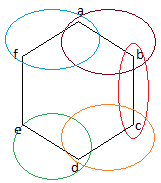
\includegraphics[width=20mm]{esboco4}
\caption{Segundo grafo com comunidades\label{fig:esb4}}
\end{figure}
\end{document}